%!TEX root = ../dokumentation.tex

\chapter{Implementierung des Tools}

\section{Grundstruktur der Applikation}

Die Grundstruktur der Applikation basiert auf zwei im MATLAB App Designer erstellten Applikationen. Der Hauptapplikation, welche das Aufrufen einzelner Funktionalität ermöglicht, sowie den Graphen der erstellen Visualisierungen darstellt, und die Applikation zur Konfiguration der Samples, welche parallel zur Hauptapplikation als Pop-Up geöffnet werden kann, jedoch nicht ohne diese verwendbar ist. Als dritte Struktur wurde die sogenannte WithSamplesParser-Klasse erstellt, welche alle Funktionalitäten bezüglich der Messdatenverarbeitung und Darstellung enthält. Dazu gehören das Einlesend und Umstrukturieren der Messdaten auf ein passendes Format, sowie das Erstellen eines Graphen mit der passenden Konfiguration. Diese Funktionen werden dabei ebenfalls aus der Hauptapplikationen gestartet und benötigen diese deshalb auch als Grundlage.

\begin{figure}[!htbp]
	\centering
	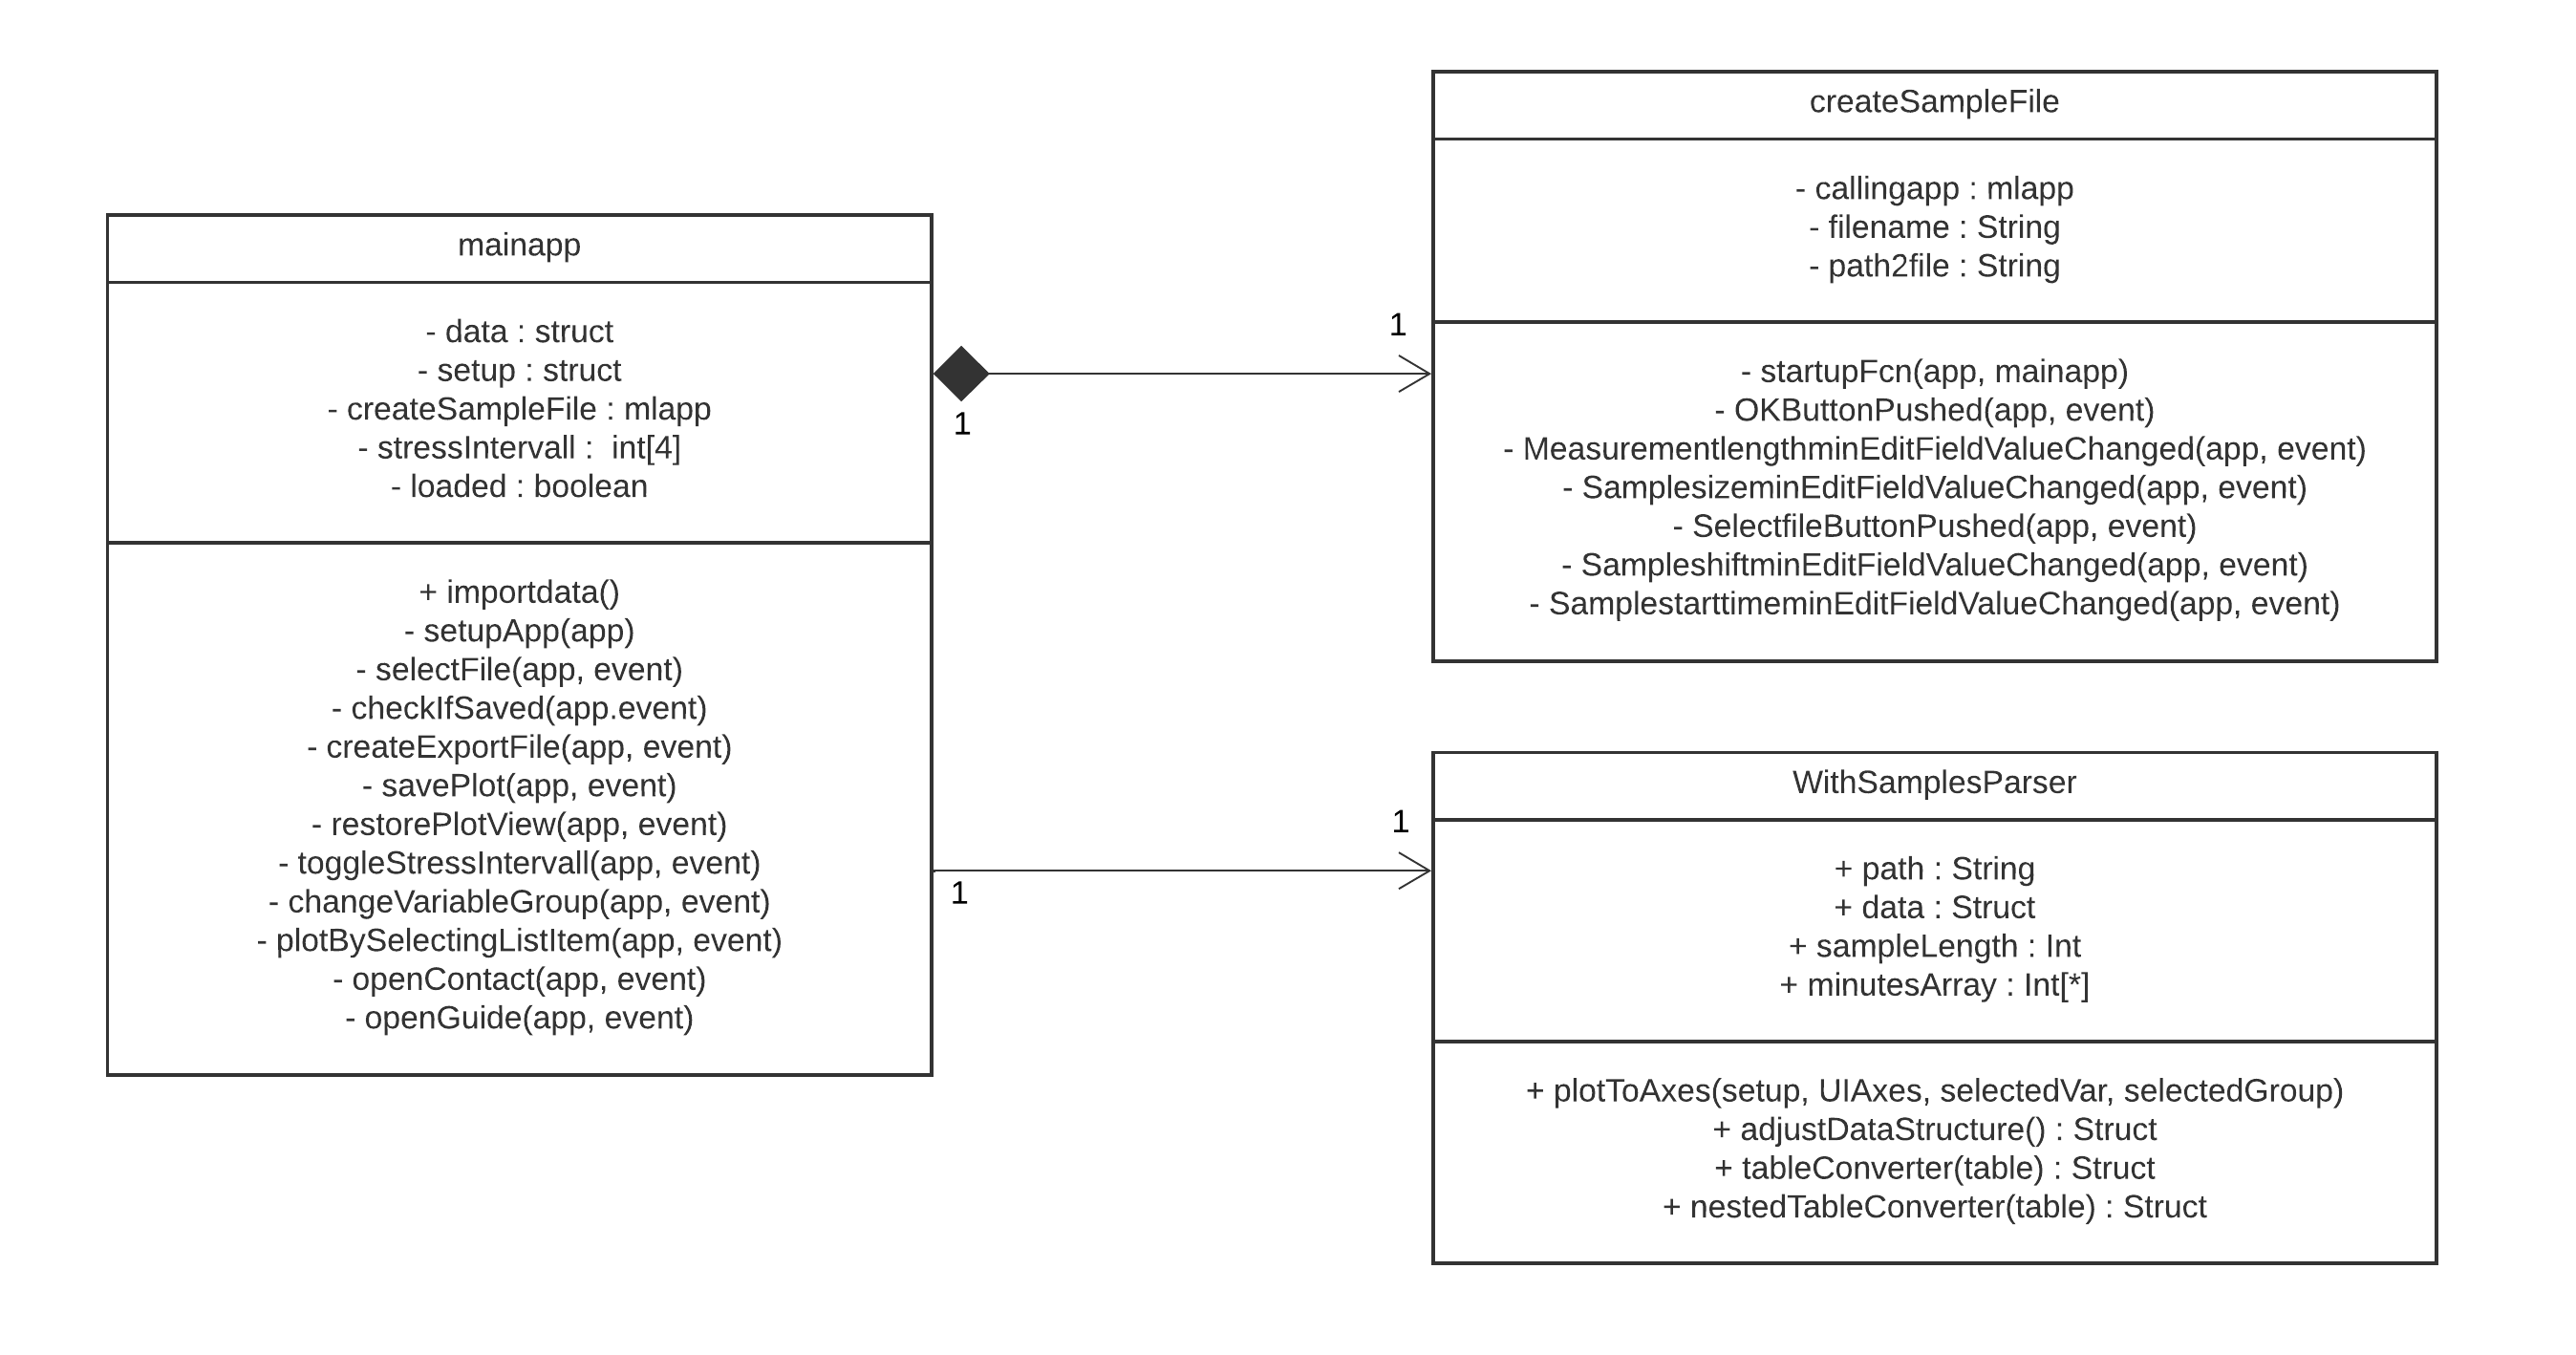
\includegraphics[width=1\linewidth]{klassendiagramm}
	\caption{Klassendiagramm der fertigen Applikation}
	\label{fig:klassendiagramm}
\end{figure}

\subsection{Layout und Komponenten}

Der MATLAB App Designer setzt bei der Erstellung von Applikation auf Code-Generierung. Der App Designer ist eine eigenständige MATLAB Applikation, welcher über eine Auswahl bereits vorgefertigter Komponenten, wie verschiedene beispielsweise Buttons, Container oder Eingabefelder verfügt. Um eine Applikation zu erstellen, können diese einfach beliebig kombiniert und visuell angepasst werden. Aus den verwendeten Komponenten wird dann eine Klasse generiert, welche beim Ausführen instanziiert wird. Diese Klasse enthält einen genauen \glqq Bauplan\grqq{} der späteren Applikation. Funktionen, welche beispielsweise durch das Klicken eines Buttons ausgelöst werden basieren auf sogenannten \textbf{Callbacks} (siehe Setup der Applikation). Diese werden direkt als Methoden der App-Klasse definiert und können nicht generiert werden. Jede Komponente kann mehrere dieser Callbacks besitzen.

\lstinputlisting[language=Matlab,numbers=left,firstline=1,lastline=8,caption={Auszug einiger verwendeter App-Komponenten}]{code/appComponents.m}

Die Grundstruktur der implementierten Applikation bildet ein \textbf{Grid-Layout}. Dies ermöglicht das korrekte Positionieren der einzelnen Komponenten innerhalb der Applikation und damit auch die symmetrische Konsistenz von Rahmen- und Komponentenabständen, welche im grundlegenden Design-Konzept definiert wurden. Außerdem fügt es der Applikation eine umfassende Responsiveness hinzu, wodurch das Verwenden der Applikation in unterschiedlichen Monitorgrößen und Fenstergrößen ermöglicht werden kann.



\todo{Die Applikation besteht aus den folgenden Elementen... (UIAxes, ListBox, etc.)}


\todo{Bild der fertigen Applikation}

\section{Setup der Applikation}

\todo{Was passiert alles beim Start der Applikation?}

\section{Erstellung der Samples}

\todo{Wim schreibt was er gemacht hat :)}
\todo{Die Applikation besteht aus den folgenden Elementen... (UIAxes, ListBox, etc.)}

\section{Visualisierung der Daten}

Im folgenden Teil der Implementierung sollen die einzelnen Schritte und Funktionen dargestellt werden, welche zum schlussendlichen Visualisieren und Auswerten der Daten beitragen. Dazu gehören die Verarbeitung der Daten und die Datenstruktur im Backend der Applikation, sowie das Darstellen des Graphen mit Hilfe der Plot-Funktion und die dazugehörigen erweiternden Funktionen wie beispielsweise das Hervorheben des Belastungsintervalls.

\subsection{Datenstruktur und Datenverarbeitung}



% möglicherweise Datenstruktur als Baumdiagramm im Anhang anfügen

\subsection{Plot-Funktion}

Die Hauptaufgaben der Plot-Funktion (dt. graphisch darstellen) sind das Auswählen des richtigen Datensatzes anhand einer gegebenen Gruppe und dem zugehörigen Messparameter, sowie das Verknüpfen der Daten mit dem Koordinatensystem und das Anpassung der Koordinatenachsen auf den passenden Stand.

Die Plot-Funktion wird dabei durch das Auswählen eines Messparameters in der Liste aller konfigurierten Parameter aufgerufen. Als Methode der Parser-Klasse \textbf{WithSampleParser} hat sie direkten Zugriff auf die eingelesenen Messdaten. Sie erhält dabei die setup-Konfiguration, das Koordinatensystem als UIAxes-Objekt des App Designers, den ausgewählten Parameter und dessen Gruppe. Zu Beginn wird anhand der übergegebenen Gruppe, der Link auf die passende Setupstruktur und die Tabelle in der Datenstruktur ermittelt.

\lstinputlisting[language=Matlab,numbers=left,firstline=1,lastline=4,caption={Beispiel der Link-Zuordnung für Parameter-Gruppe}]{code/getGroupPlot.m}

Mit den beiden Links wird nun nach dem speziellen Parameter gefiltert und dessen Index innerhalb der Tabelle zurückgegeben. Hiermit lassen sich nun das Daten-Array, der vollständige Bezeichner, die Kurzbeschreibung und die Einheit des Parameters bestimmen. 

\lstinputlisting[language=Matlab,numbers=left,firstline=1,lastline=8,caption={Index des Parameters und dazugehörige Informationen filtern}]{code/getIndexPlot.m}

Das Daten-Array wird nun als Liste der y-Werte dem Koordinatensystem übergeben und dort als Datensatz hinterlegt. Die passenden Werte der x-Achse wurden bereits innerhalb des Einlesevorgangs der Messdaten ermittelt und repräsentieren die Länge der Messung als relative Minutenangabe. Diese werden ebenfalls mit an das Koordinatensystem angehängt. Mit Hilfe der MATLAB-eigenene Scatter-Funktion wird dem UIAxes-Objekt die Information übertragen, dass es sich um einen Scatter-Plot (dt. Streu-Graphen) handelt und die x- und y-Werte-Paare als Punkte ohne verbindende Linie dargestellt werden sollen. Hier können ebenfalls Konfigurationen für die Darstellung der Daten-Tupel im Graphen übergeben werden.

\lstinputlisting[language=Matlab,numbers=left,firstline=1,lastline=4,caption={MATLAB Scatter-Funktion}]{code/plotFunktion.m}

Im letzten Schritt wird das Aussehen des Koordinatensystems angepasst, so dass es die wichtigen Informationen wie Achsenbeschriftungen aber auch Titel und Kurzbeschreibung enthält und der Bildausschnitt angenehm für den Ersteindruck ist.

\subsection{Zusätzliche Funktionen}

\todo{Belastungsintervall, Plot speichern, Plot Restoren}